\documentclass[UTF8]{ctexart}
\usepackage{CJKutf8}
\usepackage{graphicx}
\usepackage{amsmath}
\usepackage{xcolor}
\usepackage{float}
\usepackage{cite}
\usepackage{indentfirst}

  \author{黄晃 数院 1701210098 }
  \title{统计学习第一次上机作业}
\begin{document}
  \maketitle
  \section{结果}
  \subsection{问题一}
  n=100,p=5000.
  $$\beta_i=(-1)^{i}exp(-2*(i-1)/20), x_i ~ N(0,1)$$
  $$ y=X\beta+kz$$
  .其中$z~N(0,1)$,取k使得SNR=3.基于matlab实现了对偶问题的ADMM方法,作为对照,使用matlab中的cvx包进行了对应问题的求解.
  \paragraph{$\lambda$ 的选取}
  $\lambda-min=1e-3,\lambda-max=1,\lambda_i = \lambda-min*10^{(i-1)*3/100}$
  \subsubsection{solution-path}
  
\begin{figure}[H]
  \centering
  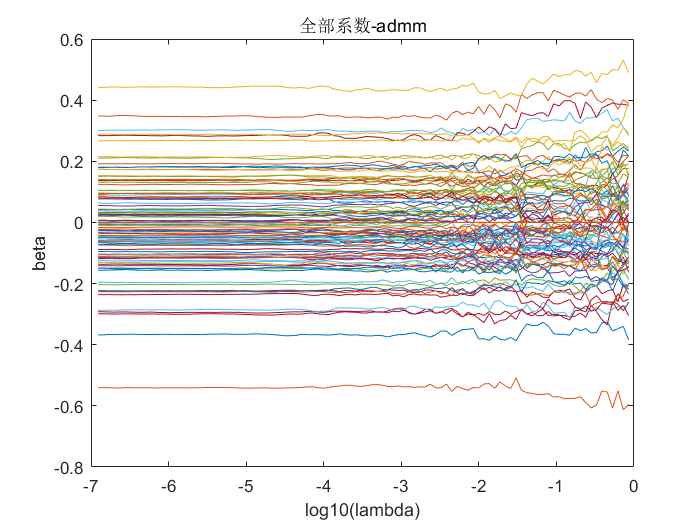
\includegraphics[width=0.45\textwidth]{admm5000.png}
  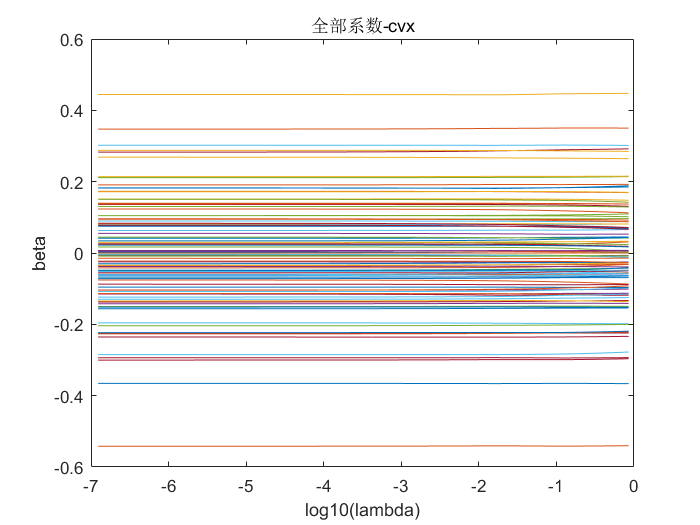
\includegraphics[width=0.45\textwidth]{cvx5000.png}
  \caption{solution path}\label{5000}
\end{figure}
  \begin{figure}[H]
  \centering
  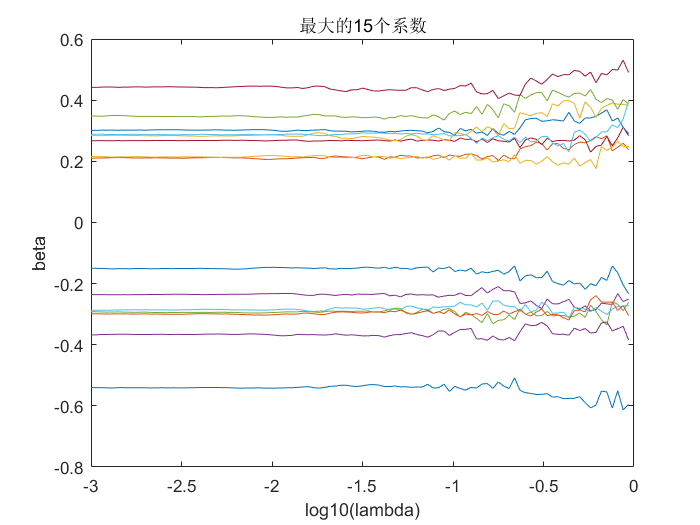
\includegraphics[width=0.45\textwidth]{admm15.png}
  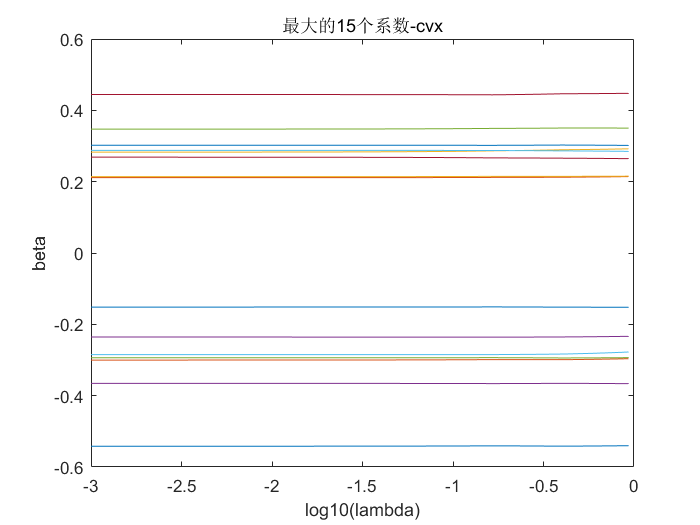
\includegraphics[width=0.45\textwidth]{cvx15.png}
  \caption{solution path (15个最大的$\beta$)}\label{15}
\end{figure}

\subsubsection{与cvx的相对误差及cpu时间}
算法以最大步长以及变量的下降量作为终止准则.F为目标函数,定义相对误差为:
$$
err=\frac{(F(x0)-F(x1))}{F(x1)}
$$
其中x1是通过cvx得到的解.
\begin{figure}[H]
  \centering
  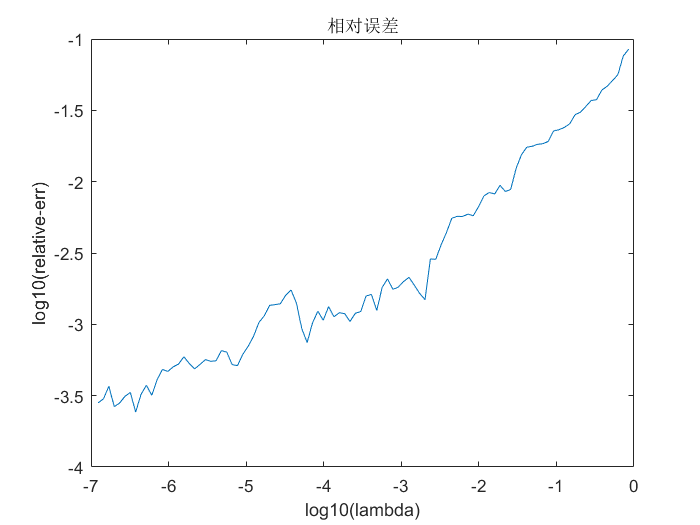
\includegraphics[width=0.45\textwidth]{err.png}
  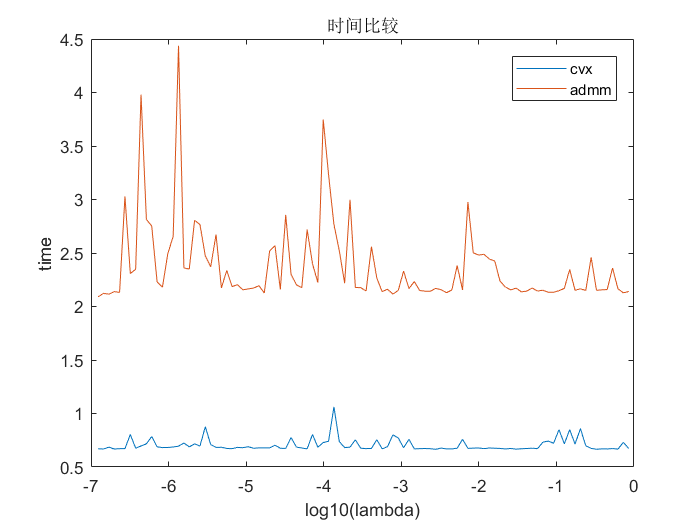
\includegraphics[width=0.45\textwidth]{time.png}
  \caption{error and time}\label{err}
\end{figure}
  \subsubsection{小结}
  \begin{itemize}
    \item 根据图一,可以看到实现的admm有稀疏性,并且结果和cvx的相似.
    \item 由图三,admm正确的求解了问题,并且在$\lambda$较小时求解精确(相对误差1e-4).但在$\lambda$较大时误差开始变大
    \item admm的时间花费在cvx的4-6倍左右.
  \end{itemize}
  \paragraph{分析以及可能改进的地方}
  上面提到的误差变大的问题,可能产生于admm方法的参数选取(现在是选择的统一的t,没有随着$\lambda$变化).算法内部的参数t根据$\lambda$变化可能会有改进.
  
  
  \subsection{问题二}
  
  
  
  \section{算法}
  \subsection{Lasso For Linear Regression}
  原问题为
  \begin{equation}\label{p:1}
    \begin{split}
       min\  & \frac{1}{2}\|Ax-b +x_0*\vec{1}\|_{2}^{2} + \mu \|x\|_{1} \\
    \end{split}
  \end{equation}
  其中$x=[x_1,x_2,\cdots,x_p]^T$

  \subsubsection{ALM求解对偶问题}
  \paragraph{对偶问题}
  首先将原问题转化为对偶问题,做线性变换
    \begin{equation}
    \begin{split}
       min\  & \frac{1}{2}\|y\|_{2}^{2} + \mu \|x\|_{1} \\
       s.t \ & y=Ax-b+x_0*\vec{1}.\\
    \end{split}
  \end{equation}
  对应的lagrangian函数为
$$
L(x,y,\lambda)=\frac{1}{2}\|y\|_{2}^{2} + \mu \|x\|_{1}-\lambda^{T}(Ax-b-y+x_0*\vec{1})
$$
直接可求得
$$
g(\lambda)= -\frac{1}{2}\|\lambda\|_{2}^{2} + \lambda^{T}b\
$$
$$
\|A^{T}\lambda\|_{\infty}\leq \mu,\ \lambda^T*\vec{1}=0
$$
所以对偶问题(D)可写作
    \begin{equation}
    \begin{split}
       min\  & \frac{1}{2}\|\lambda\|_{2}^{2} - \lambda^{T}b \\
       s.t \ & |A^{T}\lambda\|_{\infty}\leq \mu.\\
           \ &  \lambda^T*\vec{1}=0  \\
    \end{split}
  \end{equation}
\paragraph{对偶的增广lagrangian函数}
引入变量s,$A^{T}\lambda=s,\|s\|_{\infty}\leq \mu$,则对应的增广lagrangian函数为
$$
L_{t}(\lambda,s,x) = \frac{1}{2}\|\lambda\|_{2}^{2} - \lambda^{T}b + x^{T}(A^{T}\lambda-s)+\frac{t}{2}\|A^{T}\lambda-s\|_{2}^2,\  s_k\leq \mu,\  \lambda^T*\vec{1}=0
$$

由增广Lagrangian方法,我们需要:对于给定的x,求$s,\lambda$极小化$L_{t}(\lambda ,s,x)$.
\paragraph{s的求解}
在此对c进行非精确的求解,即在全空间求极小,然后在C上对s做投影.利用一阶条件,这等价于
  $$
  s_{i}=\left\{
  \begin{aligned}
   \mu & \  ,if \phi(\lambda,x)_i>\mu \\
    -\mu &\ ,if \phi(\lambda,x)_i<-\mu \\
    \phi(\lambda,x) &\ ,  else
  \end{aligned}
  \right.
$$
$$
  \phi(\lambda,x) = A^T\lambda+\frac{x}{t}
  $$
\paragraph{$\lambda$的求解}
  $\lambda$为问题
    \begin{equation}\label{p:1}
    \begin{split}
       min\  & \frac{1}{2}\|\lambda \|_{2}^{2} - \lambda^T b + x^TA^T\lambda+\frac{1}{2}t\lambda^TA^TA\lambda-t\lambda^TAs\\
       sub\  & \lambda^T*\vec{1}=0
    \end{split}
  \end{equation}
  考虑其对偶问题,引入对偶变量$\psi$
  Lagrandian方程为
  $$
  L=\frac{1}{2}\|\lambda \|_{2}^{2} - \lambda^T b + x^TA^T\lambda+\frac{1}{2}t\lambda^TA^TA\lambda-t\lambda^TAs+\psi (\lambda^T*\vec{1})
  $$
  $$
  g(\psi)=\min\limits_{\lambda} L(\lambda,\psi)
  $$
  而
  $$
  \frac{\partial L}{\partial \lambda} = (tA^TA+I)\lambda - (tAs-Ax+b-\psi*\vec{1})
  $$
  取$\lambda=(tA^TA+I)^{-1}(tAs-Ax+b-\psi*\vec{1})$得
  $$
  g(\psi)=-\frac{1}{2}(tAs-Ax+b-\psi*\vec{1})^T(tA^TA+I)^{-1}(tAs-Ax+b-\psi*\vec{1})
  $$
  由一阶条件可知
  $$
  \psi=\frac{\vec{1}^T(tA^TA+I)^{-1}(tAs-Ax+b)}{\vec{1}^T(tA^TA+I)^{-1}\vec{1}}
  $$

  显式的按上列顺序计算$s^+,\lambda^+$,然后更新x
  $$
  x^+ = x+t(A^T\lambda-s)
  $$
  综上,算法可以描述为
  $$
  \begin{aligned}
   s =& \  \min(\max(\phi(\lambda,x),-\mu),\mu) \\
   \psi =& \ \frac{\vec{1}^T(tA^TA+I)^{-1}(tAs-Ax+b)}{\vec{1}^T(tA^TA+I)^{-1}\vec{1}}   \\
   \lambda = & \  (tA^TA+I)^{-1}(tAs-Ax+b-\psi*\vec{1}) \\
   x =&\  x+t(A^T\lambda-s).
  \end{aligned}
  $$
  对应到原问题的变量,
  $$
  y = -\lambda
  $$
$$
x0=mean(y-Ax+b)
$$

  \end{document} 